
%***************************************************************************
%
% CreditCruncher - A portfolio credit risk valorator
% Copyright (C) 2004 Gerard Torrent
%
% This program is free software; you can redistribute it and/or
% modify it under the terms of the GNU General Public License
% as published by the Free Software Foundation; either version 2
% of the License.
%
% This program is distributed in the hope that it will be useful,
% but WITHOUT ANY WARRANTY; without even the implied warranty of
% MERCHANTABILITY or FITNESS FOR A PARTICULAR PURPOSE.  See the
% GNU General Public License for more details.
%
% You should have received a copy of the GNU General Public License
% along with this program; if not, write to the Free Software
% Foundation, Inc., 59 Temple Place - Suite 330, Boston, MA 02111-1307, USA.
%
%
% implementation.tex - TeX documentation file
% --------------------------------------------------------------------------
%
% 2005/01/22 - Gerard Torrent [gerard@fobos.generacio.com]
%   . initial release
%
%***************************************************************************

\chapter{Implementaci\'on}
\label{sec:implementation}


\section{Interpretaci\'on del fichero de entrada}

El contenido esperado del fichero de entrada se encuentra
descrito en el documento \emph{CreditCruncher - Input File Reference}
que se adjunta junto al programa.
\newline
\newline
El fichero de entrada puede tener un tama\~no considerable. Por
este motivo la interpretaci\'on del fichero xml se realiza usando un
sistema orientado a eventos (tipo SAX). A continuaci\'on se
describen algunas de las validaciones mas importantes:

\paragraph{Formato.} Se verifica que se trata de un fichero XML
v\'alido que cumple la DTD. V\'ease \emph{W3C}\footnote{http://www.w3.org/XML/}
para m\'as informaci\'on relativa al formato XML.

\paragraph{Valores.} Cada valor tiene un tipo (int, long, double,
date, boolean o string), un rango de valores permitidos y un
indicador de obligatorio/opcional. Para cada valor se comprueba
que se cumplen los criterios descritos en
\emph{CreditCruncher - Input File Reference}.

\paragraph{Consistencia.} Cuando un valor se refiere a un identificador,
se comprueba que el objeto referenciado existe. Por ejemplo, cuando se
lee una transici\'on en la definici\'on de la matriz de transici\'on se
comprueba que los ratings han sido definidos anteriormente y que los
ratings referenciados existen.

\paragraph{Matriz de transici\'on.} Al leer la matriz de transici\'on
se verifica que cumple con las propiedades indicadas en
\ref{sec:mtransition:properties}.

\paragraph{Funci\'on de supervivencia.} En caso de estar definida
una funci\'on de supervivencia, se comprueba que se trata de una
funci\'on positiva mon\'otona decreciente que vale $1$ cuando $t=0$,
(excepto para el rating $Default$ para la que siempre vale $0$).

\paragraph{Matriz de correlaci\'on.} Se comprueba que se trata de
una matriz sim\'etrica (por comodidad, puede entrarse solamente
el triangulo superior, o inferior), con valores comprendidos
en $[-1,+1]$.

\paragraph{Criterios de parada.} Se comprueba que exista alg\'un
criterio de parada y que este sea realizable.

%---------------------------------------------------------------------------

\section{Particionamiento del tiempo}

Para realizar el particionamiento del tiempo se necesita la fecha inicial, $t_0$,
la longitud (en meses naturales) de cada intervalo, $StepLength$, y el n\'umero
de pasos a considerar, $NumSteps$. Las fechas de la partici\'on son:
\begin{displaymath}
t_i = t_0 + i \cdot StepLength \qquad i \in \{0, 1, 2, \cdots, NumSteps\}
\end{displaymath}

Entendemos que a\~nadir $n$ meses a una fecha consiste en incrementar el
mes de la fecha inicial en $n$ meses, realizando un incremento de a\~no si
es preciso. Si el d\'ia de la fecha inicial no existe en el mes de la fecha
final, consideramos como d\'ia de la fecha final el m\'aximo d\'ia del mes
de la fecha final, en caso contrario, el mismo d\'ia de la fecha inicial.
\newline
\newline
Supongamos que $t_0=30/10/2004$, $StepLength=2$ y $NumSteps=6$, entonces la
partici\'on del tiempo es: $t_0=30/10/2004$, $t_1=30/12/2004$, $t_2=28/02/2005$,
$t_3=30/04/2005$, $t_4=30/06/2005$, $t_5=30/08/2005$ y $t_6=30/10/2005$.
Obs\'ervese como el d\'ia del mes de Febrero es el $28$ por no existir los
d\'ias $29$ y $30$ de dicho mes.

\begin{figure}[!hb]
\begin{center}
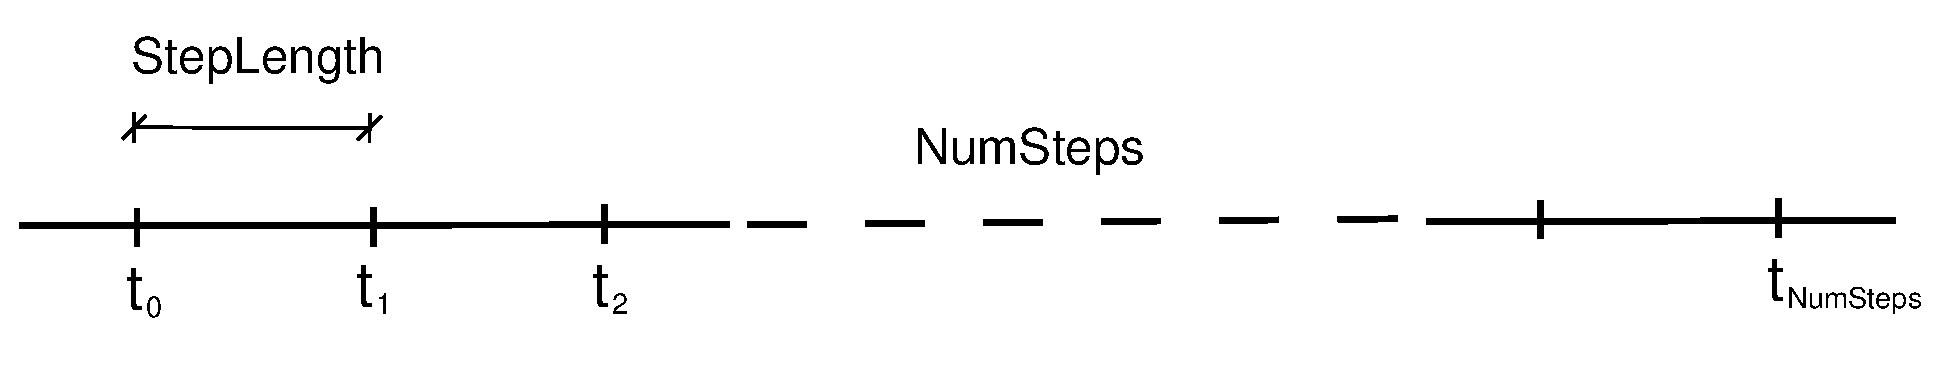
\includegraphics[width=10cm,angle=0]{./images/time.eps}
\caption{Particionamiento del tiempo}
\label{timetranches}
\end{center}
\end{figure}

%---------------------------------------------------------------------------

\section{Inicializaci\'on de los clientes}

Los clientes de la cartera se ordenan en funci\'on de su sector
y rating de forma creciente en ambos casos. La finalidad de esta
ordenaci\'on es disponer de una matriz de correlaci\'on entre
clientes en bloques. En el caso que solamente se desee simular
los clientes activos (aquellos que tienen alg\'un producto activo
durante el periodo simulado), los clientes inactivos son
suprimidos.
\newline
\newline
Supongamos que tenemos 3 sectores, S1, S2 y S3 y un sistema de
ratings compuesto por las clasificaciones A, B, C, D, y E.
Supongamos que la cartera est\'a compuesta por \footnote{el
primer componente corresponde al sector del cliente, el segundo al
rating del cliente y el tercero indica si est\'a activo (1) o inactivo (0)}:
[S2,D,1], [S3,A,1], [S1,B,1], [S1,B,0], [S3,C,1], [S2,A,1], [S2,B,1], [S3,C,1],
[S1,A,1], [S2,D,1].
\newline
\newline
La cartera ordenada es:
[S1,A,1], [S1,B,1], [S1,B,0], [S2,A,1], [S2,B,1], [S2,D,1], [S2,D,1],
[S3,A,1], [S3,C,1], [S3,C,1].
\newline
\newline
Si solamente se desea simular los clientes activos, la cartera ordenada es:
[S1,A,1], [S1,B,1], [S2,A,1], [S2,B,1], [S2,D,1], [S2,D,1], [S3,A,1],
[S3,C,1], [S3,C,1].
\newline
\newline
El n\'umero de clientes considerado es el n\'umero de clientes de la cartera.
Si solamente se est\'a simulando los clientes activos, entonces el n\'umero
de clientes considerado es el n\'umero de clientes activos.

%---------------------------------------------------------------------------

\section{Inicializaci\'on del m\'etodo de simulaci\'on}

\begin{figure}[!hb]
\begin{center}
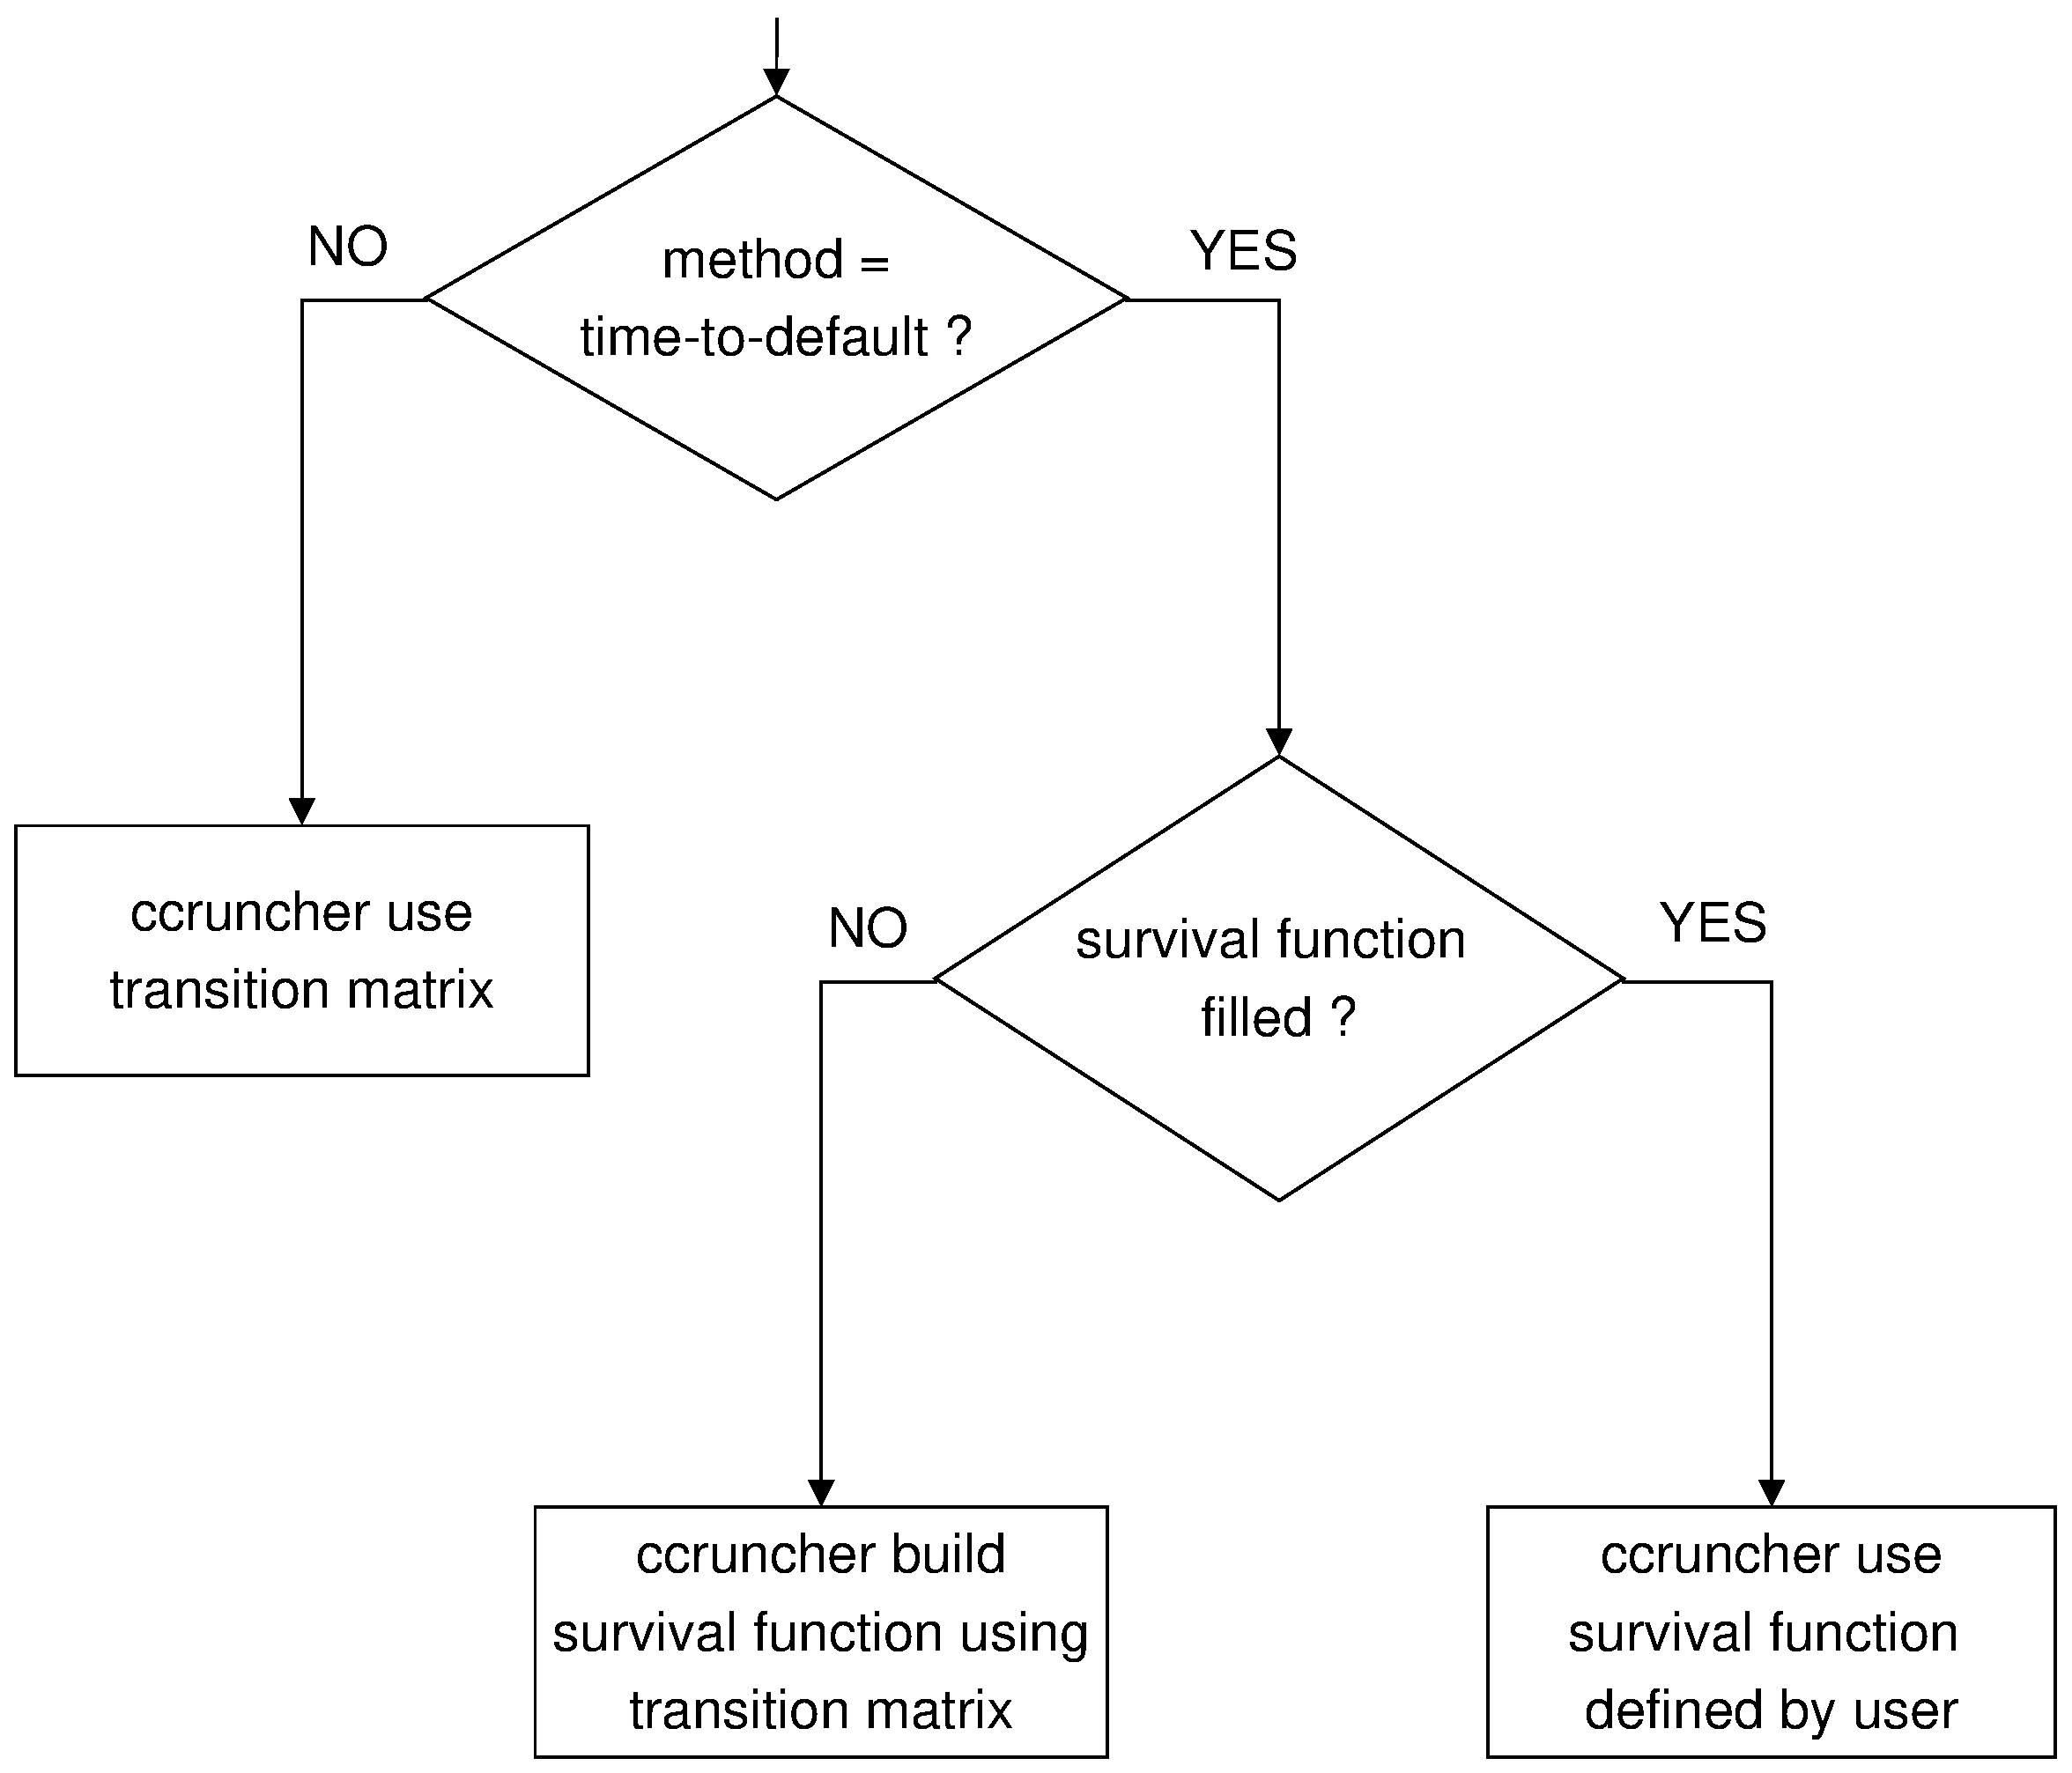
\includegraphics[width=8cm,angle=0]{./images/decisiontree1.eps}
\caption{Decisi\'on en funci\'on del m\'etodo}
\label{decisiontree1}
\end{center}
\end{figure}

\subsection{M\'etodo Rating-Path}

El m\'etodo Rating-Path requiere disponer de la matriz de transici\'on
para el periodo $StepLength$. A partir de la matriz de transici\'on
definida por el usuario para el periodo T (normalmente 1 a\~no), se
construye la matriz de transici\'on para el periodo $StepLength$ usando
las indicaciones de \ref{mtrans:perchange}.
\begin{displaymath}
M_{StepLength} = M_{T}^{\frac{StepLength}{T}} = \sqrt[T]{M_{T}^{StepLength}}
\end{displaymath}

El algoritmo para calcular la ra\'iz de una matriz a partir de la matriz
de autovectores y sus autovalores est\'a explicado en el ap\'endice
\ref{apendix:sqrtmat}.

\subsection{M\'etodo Time-To-Default}

El m\'etodo Time-To-Default requiere disponer de la funci\'on de
supervivencia. Si el usuario ha definido una se considera la
funci\'on de supervivencia definada por el usuario. En caso
contrario se construye a partir de la matriz de transici\'on
usando las indicaciones de \ref{mtrans:survival}.

\begin{displaymath}
Survival(r_i,t_j) = 1 - (M_{StepLength}^j)_{i,n} \qquad j \in \{0,1,2,\cdots,NumSteps\}
\end{displaymath}
donde $(M_{StepLength}^j)_{i,n}$ debe interpretarse como la columna $n$ de
la fila $i$ de la matriz $M_{StepLength}$ elevada a $j$. La matriz de transici\'on
para el periodo $StepLength$, $M_{StepLength}$, se determina a partir de la matriz
de transici\'on proporcionada por el usuario para el periodo T (normalmente 1 a\~no)
usando las indicaciones de \ref{mtrans:perchange}.
\begin{displaymath}
M_{StepLength} = M_{T}^{\frac{StepLength}{T}} = \sqrt[T]{M_{T}^{StepLength}}
\end{displaymath}
El algoritmo para calcular la ra\'iz de una matriz a partir de la matriz
de autovectores y sus autovalores est\'a explicado en el ap\'endice
\ref{apendix:sqrtmat}.

%---------------------------------------------------------------------------

\section{Inicializaci\'on de las c\'opulas}

Los pasos 1 y 2 de \ref{apendix:gaussiancopula} explican como
inicializar una c\'opula gaussiana. CreditCruncher aplica el 
mismo algoritmo, pero teniendo en cuenta que la matriz de
correlaci\'on entre clientes es una matriz en bloques. Esto
permite un ahorro de memoria y tiempo de c\'alculo. En vez de
considerar la matriz de correlaci\'on entre clientes se
considera la matriz de correlaci\'on entre sectores y el
n\'umero de clientes en cada sector. Se aplica el paso 1
de \ref{apendix:gaussiancopula} a la matriz de correlaci\'on
entre sectores. Se reemplaza el paso 2 de \ref{apendix:gaussiancopula}
por \ref{apendix:cholblock}.


\subsection{M\'etodo Rating-Path}

Si el m\'etodo de simulaci\'on es el Rating-Path se construyen
$NumSteps$ c\'opulas. La primera c\'opula se usar\'a para simular
los cambios de rating entre $t_0$ y $t_1$, la segunda c\'opula
para simular los cambios de rating entre $t_1$ y $t_2$, etc.
\newline
\newline
El generador de n\'umeros aleatorios de cada c\'opula se
inicializa con la siguiente semilla:
\begin{displaymath}
Seed(i,q) = Seed(1,0) + q \cdot 30001 + (i-1)
\end{displaymath}
donde $Seed(i,q)$ es la semilla del generador de n\'umeros de la
c\'opula $i$ de la instancia $q$ (en el caso de ejecutarse en un
cluster $q>0$, en caso contrario, $q=0$). $Seed(1,0)$ es la semilla
proporcionada por el usuario (un n\'umero aleatorio si el usuario no
especifica semilla o especifica una semilla igual a 0). De esta
forma se garantiza que todas las instancias usan una semilla distinta
(siempre que el n\'umero de instancias mas $NumSteps$ no supere 30000).

\subsection{M\'etodo Time-To-Default}

Si el m\'etodo de simulaci\'on es el Time-To-Default se construye
1 c\'opula. Se usar\'a para simular el tiempo de fallido.
\newline
\newline
El generador de n\'umeros aleatorios de cada c\'opula se
inicializa con la siguiente semilla:
\begin{displaymath}
Seed(1,q) = Seed(1,0) + q \cdot 30001 + 0
\end{displaymath}
donde $Seed(i,q)$ es la semilla del generador de n\'umeros de la
c\'opula $i$ de la instancia $q$ (en el caso de ejecutarse en un
cluster $q>0$, en caso contrario, $q=0$). $Seed(1,0)$ es la semilla
proporcionada por el usuario (un n\'umero aleatorio si el usuario no
especifica semilla o especifica una semilla igual a 0). De esta
forma se garantiza que todas las instancias usan una semilla distinta
(siempre que el n\'umero de instancias no supere 30000).

%---------------------------------------------------------------------------

\section{Mapeo del cashflow}

Sea $t_0, t_1, t_2, \cdots, t_k$ la partici\'on de tiempo usada.
Dado un cashflow $(t_v,V)$ lo mapeamos en la estructura
temporal de la siguiente forma:

\begin{enumerate}
\item Si $t_v < t_0$, entonces $(t_v,V) \longrightarrow (t_0,0)$
\item Si $t_{i-1} < t_v \leq t_i$, entonces $(t_v,V) \longrightarrow (t_i,V \cdot \Upsilon(t_v,t_i))$
\item Si $t_k < t_v$, entonces $(t_v,V) \longrightarrow (t_k,0)$
\end{enumerate}

donde $\Upsilon(t_v,t_i)$ es el coeficiente de transporte entre $t_v$ y $t_i$.

\begin{figure}[!hb]
\begin{center}
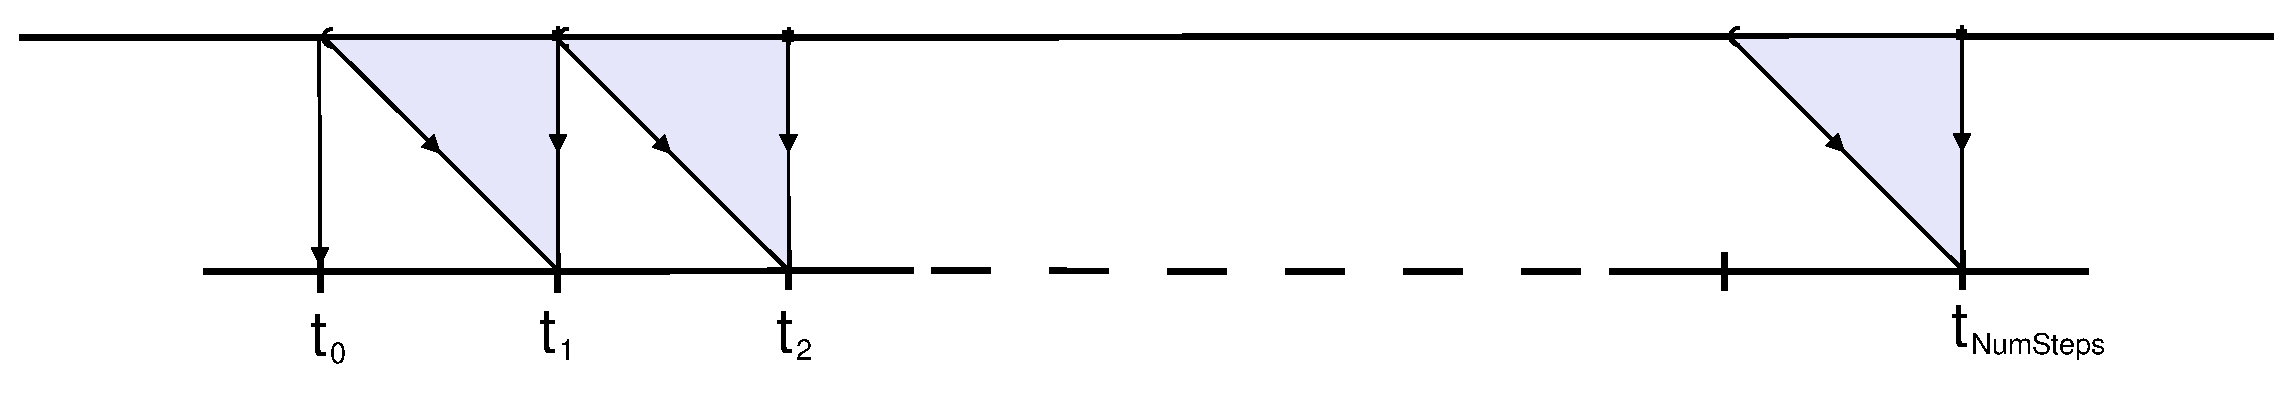
\includegraphics[width=10cm,angle=0]{./images/cashflowmapping.eps}
\caption{CashFlow mapping}
\label{timetranches}
\end{center}
\end{figure}

Veamos un ejemplo. Consideramos $\Upsilon(t_i,t_j)=1$ para no complicar los c\'alculos.
A la izquierda se representa el cashflow original (sin estar mapeado a los nodos de
tiempo). A la derecha se encuentra el mismo cashflow mapeado a los nodos de tiempo.
\newline
\newline
\begin{minipage}[c]{0.5\columnwidth}%
\centering
\begin{tabular}{c|r}
\textbf{Date} & \textbf{Cashflow} \\
\hline
17/04/2004 & -10.00 \\
           &        \\
           &        \\
05/01/2005 &   1.00 \\
20/01/2005 &   2.00 \\
           &        \\
15/03/2005 &   3.00 \\
           &        \\
           &        \\
30/08/2005 &   4.00 \\
           &        \\
15/12/2005 &   5.00 \\
\end{tabular}
\end{minipage}%
\begin{minipage}[c]{0.5\columnwidth}%
\centering
\begin{tabular}{c|c|c}
\textbf{$t_i$} & \textbf{Date}  & \textbf{Cashflow} \\
\hline
      &            &      \\
$t_0$ & 30/10/2004 & 0.00 \\
$t_1$ & 30/12/2004 & 0.00 \\
      &            &      \\
      &            &      \\
$t_2$ & 28/02/2005 & 1.00 + 2.00 \\
      &            &      \\
$t_3$ & 30/04/2005 & 3.00 \\
$t_4$ & 30/06/2005 & 0.00 \\
$t_5$ & 30/08/2005 & 4.00 \\
$t_6$ & 30/10/2005 & 0.00 \\
      &            &      \\
\end{tabular}
\end{minipage}%

%---------------------------------------------------------------------------

\section{Mapeo del netting}

Sea $t_0, t_1, t_2, \cdots, t_k$ la partici\'on de tiempo usada.
Calculamos el netting en un nodo, $t_i$, de la partici\'on de la
siguiente forma:

\begin{enumerate}
\item Si existe un netting anterior, $(t_a,W_a)$, y otro posterior, $(t_b,W_b)$,
a $t_i$, entonces el valor del netting en $t_i$ es
$A + (B-A) \cdot \frac{t_i-t_a}{t_b-t_a}$ donde
$A=\Upsilon(t_a,t_i) \cdot W_a$ y $B=\Upsilon(t_b,t_i) \cdot W_b$.
\item Si no existe un netting anterior a $t_i$ entonces el valor del netting
en $t_i$ es $0$.
\item Si existe un netting entre $t_{i-1}$ y $t_i$, $(t_a,W_a)$, pero no existe un
netting posterior a $t_i$, entonces el valor del netting en $t_i$ es
$\frac{t_a-t_{i-1}}{t_i-t_{i-1}} \cdot W_a \cdot \Upsilon(t_a,t_i)$
\end{enumerate}

\begin{figure}[!hb]
\begin{center}
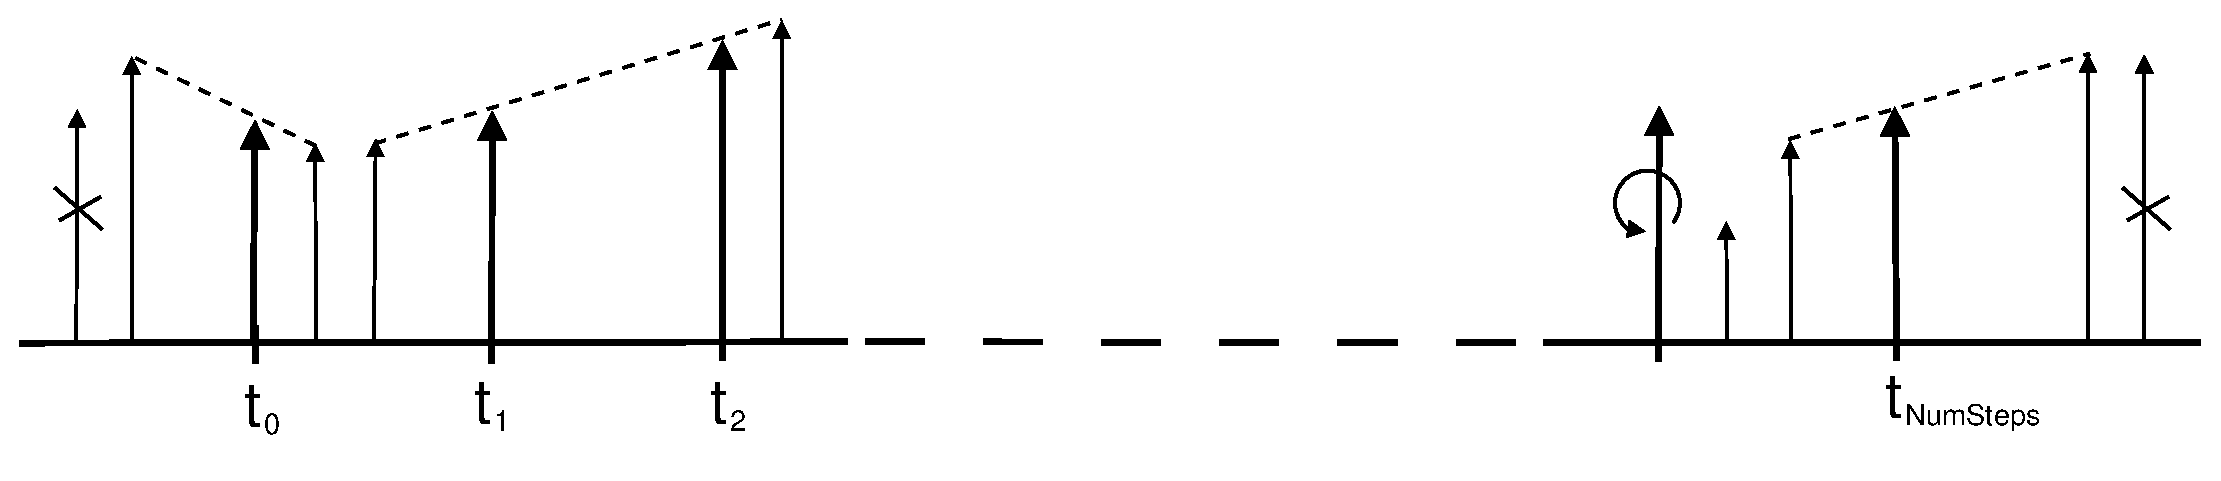
\includegraphics[width=10cm,angle=0]{./images/nettingmapping.eps}
\caption{Netting mapping}
\label{timetranches}
\end{center}
\end{figure}

Veamos un ejemplo. Consideramos $\Upsilon(t_i,t_j)=1$ para no complicar los c\'alculos.
A la izquierda se representa el netting original (sin estar mapeado a los nodos de
tiempo). A la derecha se encuentra el netting mapeado a los nodos de tiempo.
\newline
\newline
\begin{minipage}[c]{0.4\columnwidth}%
\centering
\begin{tabular}{c|r}
\textbf{Date} & \textbf{Cashflow} \\
\hline
17/04/2004 & -10.00 \\
           &        \\
           &        \\
05/01/2005 &   1.00 \\
20/01/2005 &   2.00 \\
           &        \\
15/03/2005 &   3.00 \\
           &        \\
           &        \\
30/08/2005 &   4.00 \\
           &        \\
15/12/2005 &   5.00 \\
\end{tabular}
\end{minipage}%
\begin{minipage}[c]{0.6\columnwidth}%
\centering
\begin{tabular}{c|c|c}
\textbf{$t_i$} & \textbf{Date}  & \textbf{Cashflow} \\
\hline
      &            &      \\
$t_0$ & 30/10/2004 & $-10.00 + (1+10) \cdot \frac{196}{263} =  -1.8$\\
$t_1$ & 30/12/2004 & $-10.00 + (1+10) \cdot \frac{196}{263} =  0.75$ \\
      &            &      \\
      &            &      \\
$t_2$ & 28/02/2005 & $2 + (3-2) \cdot \frac{39}{54} = 2.72$ \\
      &            &      \\
$t_3$ & 30/04/2005 & $3.00 + (4-3) \cdot \frac{46}{168} = 3.27$ \\
$t_4$ & 30/06/2005 & $3.00 + (4-3) \cdot \frac{107}{168} = 3.64$ \\
$t_5$ & 30/08/2005 & $4.00$ \\
$t_6$ & 30/10/2005 & $4.00 + (5-4) \cdot \frac{61}{107} = 4.57$ \\
      &            &      \\
\end{tabular}
\end{minipage}%

%---------------------------------------------------------------------------

\section{Inicializaci\'on del problema}


precalculo de los valores en los nodos


\section{Proceso de agregaci\'on}

TODO: descripcion de los agregadores y metodo usado para evitar recalculo 
de los activos en cada simulacion + Agregaci\'on de productos

aceleraci\'on de la convergencia usando metodolog\'ia antithetic

convergencia media, varianza, var (estimadores, graficos, etc.)
